\documentclass[t]{beamer}


\usepackage{header100}
\usepackage{header_maps}

\usepackage{amsfonts}
\usepackage{amssymb}
\usepackage{amsmath}
\usepackage{times}
\usepackage{graphicx}
\usepackage{sidecap}
\usepackage{mathtools}
\usepackage{caption}
\usepackage{breakurl}
\usepackage{bm}
\usepackage[all]{xy}
\usepackage{lipsum}
\usepackage{amsthm}
\usepackage{tikz}
\usepackage{booktabs}
\usepackage{pgfplots}
\usepackage{tabularx}
\usetikzlibrary{positioning}
\usepackage{xurl}



\DeclarePairedDelimiter\ceil{\lceil}{\rceil}
\DeclarePairedDelimiter\floor{\lfloor}{\rfloor}

\DeclareMathOperator{\cok}{coker}
\DeclareMathOperator{\im}{im}
\DeclareMathOperator{\ann}{Ann}
\DeclareMathOperator{\Hom}{Hom}

\makeatletter
\newenvironment<>{proofs}[1][\proofname]{%
 \par
 \def\insertproofname{#1\@addpunct{.}}%
 \usebeamertemplate{proof begin}#2}
 {\usebeamertemplate{proof end}}
\makeatother

\newcommand{\ik}[1]{\begin{block}{iClicker Activity} #1 \end{block}}
\newcommand{\ex}[1]{\begin{block}{Exercise} #1 \end{block}}
\newcommand{\co}[1]{[#1)}
\newcommand{\oc}[1]{(#1]}
\newcommand{\p}{\pause}
\newcommand{\ddx}{\frac{d}{dx}}
\newcommand{\eb}[1]{\begin{exampleblock}{} #1 \end{exampleblock}}
\newcommand{\RR}{\mathbb{R}}


%Information to be included in the title page:
\title{A Quick Introduction to Knots and Jones Polynomials}
\institute{University of Manitoba}
\author{Junyu Lu}
\date{Nov 2023}
\titlegraphic{
\includegraphics[height=1cm]{pic/um.png}}

\begin{document}

\frame{\titlepage}

\begin{frame}[c]
	\frametitle{Definitions}
	\begin{center}
		Knot = A piece-wise (or smooth) linear embedding of $S^1$ into $\RR^3$\\
		\p
		\vspace{0.2in}
		Link = A p.l. (or smooth) embedding of several circles into $\RR^3$
	\end{center}
	\p
	\begin{figure}
		\centering
		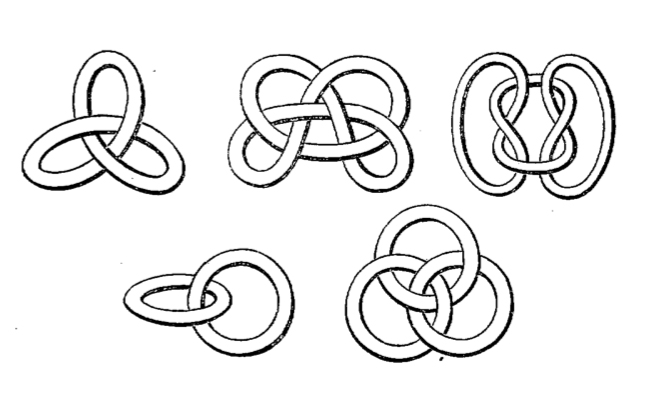
\includegraphics[width=6cm]{pic/kelvin_knots.jpg}
		\caption{Illustrations of knots and links, including a trefoil knot, top left, in an 1869 paper by Lord Kelvin on his knotted vortex theory of atoms.}
	\end{figure}
\end{frame}

\begin{frame}[c]
	\frametitle{Definitions}
	\begin{center}
		two knots are equ
	\end{center}
\end{frame}

\end{document}